\documentclass[border=0.125cm]{standalone}
\usepackage{tikz}
\usepackage{pgfplots}
\usepackage{graphicx}

\usetikzlibrary{decorations.pathmorphing}
\pgfplotsset{compat=newest}
\usetikzlibrary{shapes.geometric,arrows,fit,matrix,positioning}
\tikzset{main node/.style={circle,fill=black!20,draw,minimum size=3.5mm,inner sep=0pt},
         every node/.style={circle,fill=black,draw,minimum size=1mm,inner sep=0pt,label distance=-1mm},
         subtree/.style={isosceles triangle,fill=blue!20,draw,minimum size=4mm,inner sep=0pt,shape border rotate=90},
         edge label/.style = {rectangle,draw=none,fill=none}
}
\begin{document}
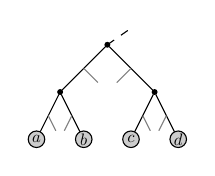
\begin{tikzpicture}[-,>=stealth', 
level 1/.style={sibling distance = 20mm},
level distance = 1cm, 
scale=0.6,
transform shape]
% \draw[help lines] (-2,2) grid (5,-5);
\node (0) {}
    child{
        [sibling distance = 10mm] node (1) {}
            child{
                node [main node] (2) {$a$}
            }
            child{
                node [main node] (3) {$b$}
            }
    }
    child{
        [sibling distance = 10mm] node (6) {}
            child{
                node [main node] (4) {$c$}
            }
            child{
                node [main node] (5) {$d$}
            }
    }
;
\draw[dashed] (0,0) -- (0.5,0.35);

\draw[gray] (0.25-1,-0.5-1) -- (0.09-1,-0.82-1);
\draw[gray] (-0.25-1,-0.5-1) -- (-0.09-1,-0.82-1);

\draw[gray] (0.25+1,-0.5-1) -- (0.09+1,-0.82-1);
\draw[gray] (-0.25+1,-0.5-1) -- (-0.09+1,-0.82-1);

\draw[gray] (6-6.5,-7.5+7) -- (6.3-6.5,-7.8+7);
\draw[gray] (0.5,-0.5) -- (6.7-6.5,-7.8+7);

\end{tikzpicture}

\end{document}






